\documentclass[11pt,letterpaper]{article}
\usepackage{graphicx}
\usepackage[english]{babel}
\usepackage{hyperref}
\usepackage{pdfpages}
\usepackage{times}
\usepackage{geometry}

\geometry{pdftex, portrait,
          headsep=8pt, headheight=8pt, footskip=16pt,
          top=88pt, bottom=88pt,
          left=72pt, right=72pt
}


\begin{document}

\title{The PENNANT Mini-App}
\author{Charles R. Ferenbaugh \\
        Los Alamos National Laboratory \\
        {\tt cferenba@lanl.gov}}
\date{Version 0.6 -- February 2014 \\
      LA-CC-12-021 \\
      \url{https://github.com/losalamos/PENNANT}}
\maketitle

PENNANT is an unstructured mesh physics mini-app designed for advanced
architecture research.
It contains mesh data structures and a few physics algorithms adapted
from the LANL rad-hydro code FLAG, and gives a
sample of the typical memory access patterns of FLAG.


\section{Building and running the code}

\subsection{Building}

A simple {\tt Makefile} is provided in the top-level directory for building
the code.  Before using it, you may wish to edit the definitions of CXX
and CXXFLAGS to specify your desired C++ compiler and flags, and to
choose between optimized/debug and serial/OpenMP/MPI builds.  Then
a simple ``{\tt make}'' command will create a {\tt build} subdirectory and
build the {\tt pennant} binary in that directory.

PENNANT has been tested under GCC 4.7.2, PGI 13.10, and Intel 13.1.3.
Building under other compilers should require only minor changes.

\subsection{Running tests}

Several test problems are provided in subdirectories under the {\tt test}
directory.  The command line
\begin{quote}
{\tt pennant \emph{testname}.pnt}
\end{quote}
is used to run a test in serial mode.  If running under MPI, this should
be preceded by {\tt mpirun} or similar command as appropriate on your
system.

The available test problems are listed in Table~\ref{tbl:tests}.
The smaller problems run quickly and are useful for debugging and
regression tests; gold standard files are provided (see next section).
The larger tests take longer to run and are suitable for timing tests.

\begin{table}
\centering
\caption{Test problems provided with PENNANT.}
\label{tbl:tests}
\begin{tabular}{lrll}
    \hline
    name & \# zones & mesh shape & zone type \\
    \hline
    Leblanc problems~\cite{leblanc}: \\
    leblanc    &    900 & rectangle & quad \\
    leblancbig & 230400 & rectangle & quad \\
    \hline
    Noh problems~\cite{noh}: \\
    nohsmall   &     40 & radial    & triangle/quad \\
    noh        &   3000 & radial    & triangle/quad \\
    nohsquare  & 129600 & square    & quad \\
    nohpoly    &  63001 & square    & mostly hexagons \\
    \hline
    Sedov problems~\cite{sedov}: \\
    sedovsmall &     81 & square    & quad \\
    sedov      &   2025 & square    & quad \\
    sedovbig   & 291600 & square    & quad \\
    \hline
\end{tabular}
\end{table}

\subsection{Test inputs and outputs}

Each test problem directory contains an input file with the {\tt.pnt}
suffix.  This is a small text file containing input parameters for the
test.

PENNANT generates output files of two kinds.  The {\tt.xy} output file
is a text file containing the per-zone values of zone density, energy,
and pressure.  (It is modeled after a similar file generated by FLAG.)
Note that, when running under MPI, the order of the output values in
this file may vary when the number of PEs changes.
For the smaller tests, two gold standard files are provided for reference.
The {\tt.xy.std} file gives the expected results for a serial run (or
1-PE MPI run), while the {\tt.xy.std4} file gives expected results for
a 4-PE MPI run.  (These files are identical except for the ordering of
zones, which is done differently depending on the number of PEs in use.)

There are also several graphics output files in Ensight Gold format:
the main file has suffix {\tt.case}, and it refers to auxiliary files
with suffixes {\tt.geo}, {\tt.ze}, {\tt.zp}, and {\tt.zr}.  These
can be viewed by the proprietary
Ensight\footnote{\url{http://www.ensight.com}}
viewer, or by open-source viewers such as
ParaView\footnote{\url{http://www.paraview.org}} and
VisIt\footnote{\url{https://wci.llnl.gov/codes/visit/home.html}}.
Sample outputs are shown in Figure~\ref{fig:output}.
\begin{figure}
    \centering
    \begin{tabular}{ccc}
    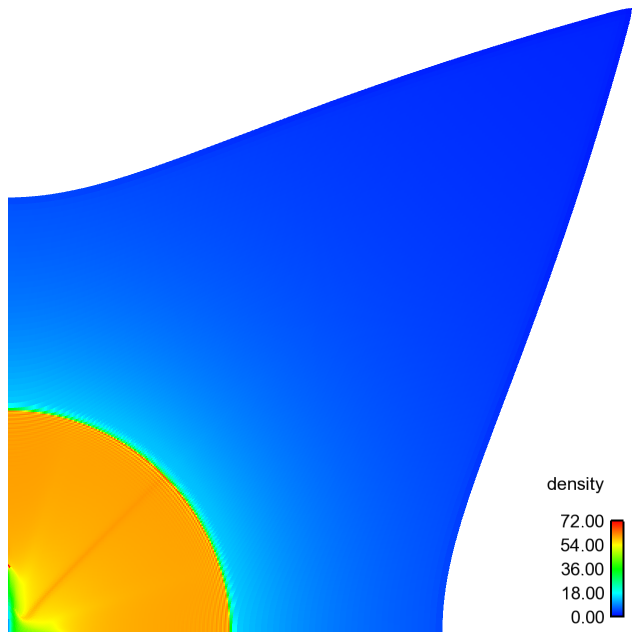
\includegraphics[width=0.40\textwidth]{noh-result.png} &
    \hspace{0.06\textwidth} &
    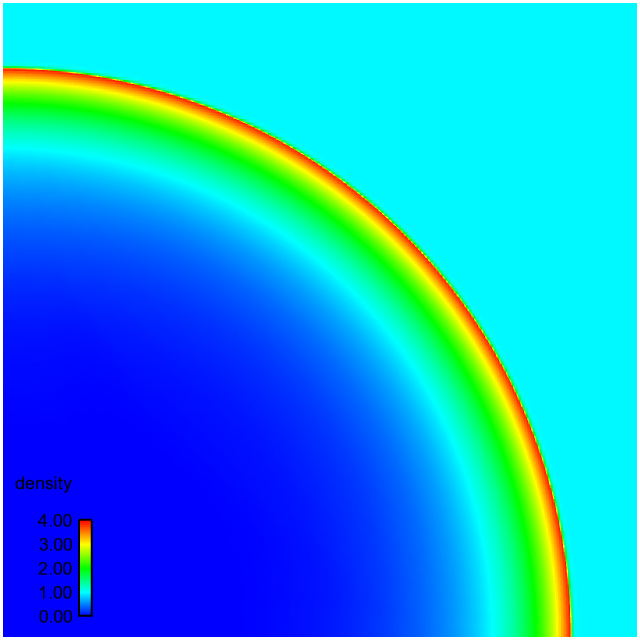
\includegraphics[width=0.40\textwidth]{sedov-result.png} \\
    (a) && (b) \\
    \end{tabular}
    \begin{tabular}{c}
    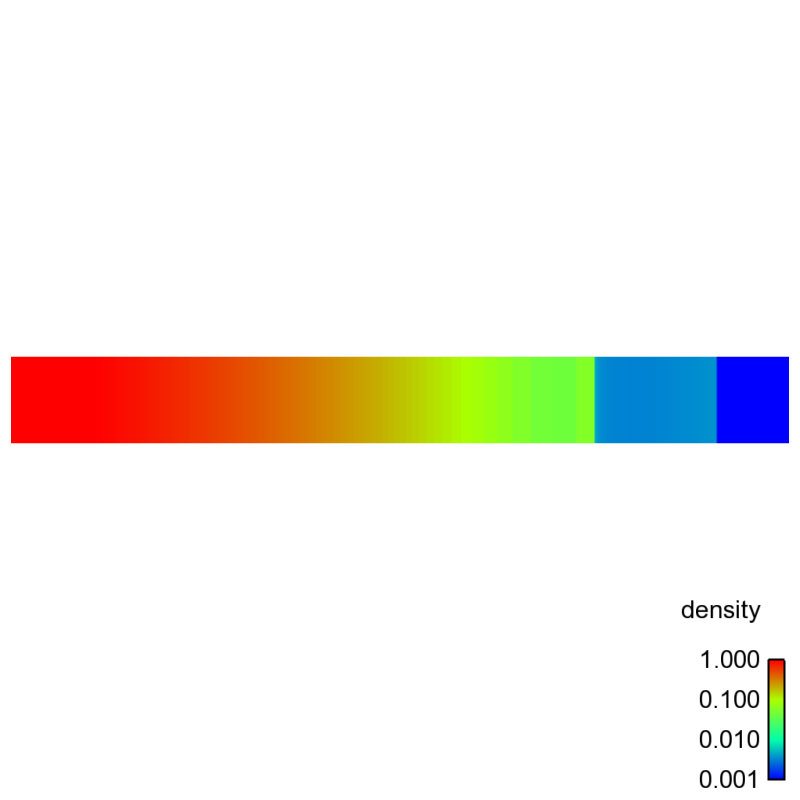
\includegraphics[width=0.40\textwidth]{leblanc-result.png} \\
    (c) \\
    \end{tabular}
    \caption{Final state of (a) {\em nohsquare}, (b) {\em sedovbig},
    and (c) {\em leblancbig} problems, colored by zone density.}
    \label{fig:output}
\end{figure}

\subsection{Input file parameters}

In most cases, there is no need for users to modify input files.  However,
here a few parameters that ambitious users might want to know about:
\begin{description}
    \item[{\tt cstop}]  Stop run when problem reaches given cycle number.
    \item[{\tt tstop}]  Stop run when problem reaches given simulation time.
    \item[{\tt chunksize}]  Process mesh elements in chunks of given size;
        see section~\ref{sec:chunk} for more details on chunk processing.
        If {\tt chunksize} is zero, the entire mesh is
        treated as a single chunk (this is the default).
        Typically, for best performance, this value will be chosen so
        that a chunk can fit in L1 or L2 cache as appropriate; it
        follows that the optimal value is architecture-dependent.
    \item[{\tt meshparams}]  Parameters for internal mesh generator.
        These may be modified if additional test cases of varying sizes are
        desired (e.g., for scaling studies).  The format of this line
        is: \\
        {\tt meshparams \emph{nzx [nzy [lenx [leny]]]}} \\
        where the parameters have the following meanings: \\
        \begin{tabular}{lp{320pt}}
            {\tt\emph{nzx, nzy}} &
            number of zones in x, y directions
            (no default for nzx; default nzy = nzx) \\
            {\tt\emph{lenx, leny}} &
            total length in x, y directions
            (default for both = 1.0, except when meshtype = pie,
            in which case default for lenx = 90.0)
        \end{tabular} \\
        For the {\em pie} mesh type, {\em x} and {\em y}
        should be understood as $\theta$ and {\em r} respectively.
    \item[{\tt dtinit}]  Initial timestep.  This shouldn't need to be
        changed unless the mesh has been changed (see
        {\tt meshparams} above).  As a rule of thumb, if the resolution
        of the problem is increased by a factor of $r$ in each direction,
        {\tt dtinit} must decrease by a factor of $r$.
\end{description}


\section{Data structure details}

\subsection{Mesh data structures}

PENNANT is designed to use standard finite-volume meshes similar to
those used by many common physics solvers.  In particular, PENNANT
supports 2-D unstructured meshes composed of arbitrary polygons.

The PENNANT mesh data structures are a subset of those used by FLAG.
These are implemented in the {\tt Mesh} class.
FLAG supports 1-, 2-, and 3-D meshes with various geometries; for
simplicity, PENNANT is restricted to the 2-D, cylindrical geometry
case.

The PENNANT terminology for entities within a mesh is shown in
Figure~\ref{fig:mesh}.  The basic mesh elements in 0, 1, and 2 dimensions
are called {\em points, edges,} and {\em zones} respectively.
PENNANT also uses two types of sub-zone entities.  Within any given
zone, a {\em side} is a triangle whose vertices are two consecutive
boundary points of the zone together with the zone center.  A {\em corner}
is a quadrilateral whose vertices are one boundary point of a zone,
the midpoints of the two adjoining edges, and the zone center.

\begin{figure}
    \centering
    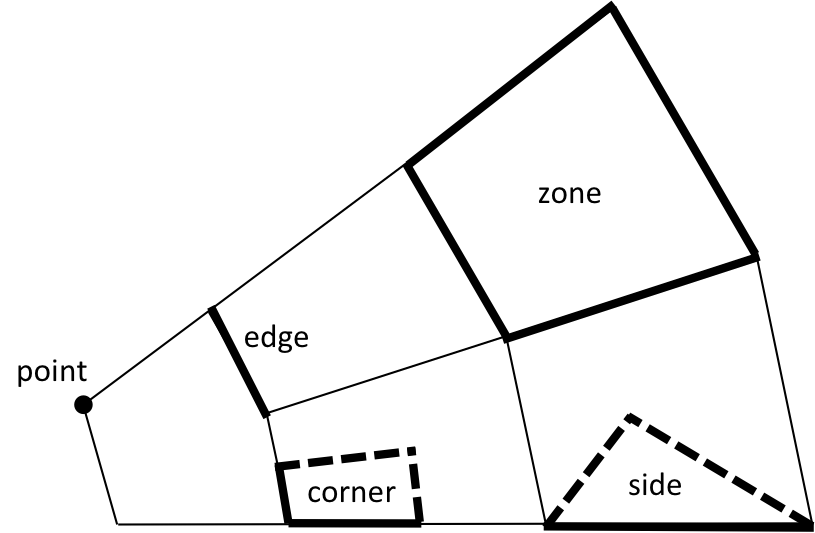
\includegraphics[width=0.50\textwidth]{mesh-entities.png}
    \caption{PENNANT terminology for mesh entities.}
    \label{fig:mesh}
\end{figure}

For each entity type, the first letter of its name is used as an
identifier for variables associated with it.  For example, {\tt px}
is an array of point coordinates, and {\tt zvol} is an array
of zone volumes.  There are scalar variables of the form
{\tt numX} which give the number of {\tt X}'s in the problem:
{\tt nump} is the number of points, and so on.

PENNANT also stores various mapping arrays from sides to other entity
types.  These are shown in Figure~\ref{fig:side}.
Given a side $s$, the following mapping arrays are available:
\begin{itemize}
\item {\tt mapsz} gives the zone $z$ of which $s$ is a subregion.
\item {\tt mapse} gives the edge $e$ on the boundary of $s$.
\item {\tt mapsp1} and {\tt mapsp2} give the two mesh points $p_1$ and
$p_2$ on the boundary of $s$.  It is assumed that the mesh is oriented
according to a right-hand rule, so that the edge from $p_1$ to $p_2$
is always in a counter-clockwise direction relative to the zone.
\item {\tt mapss3} and {\tt mapss4} give the two sides $s_3$ and
$s_4$ on either side of $s$, where $s_3$ is before $s$ and $s_4$ is
after it in a counter-clockwise traversal of the zone.
\end{itemize}
Since there is a one-to-one correspondence between sides and corners,
side-to-corner arrays are not used.  By convention, the corner labeled
$c_1$ in Figure~\ref{fig:side} has the same index as $s$.  It follows
that $c_2$ has the same index as $s_4$, or {\tt mapss4[s]}.

\begin{figure}
    \centering
    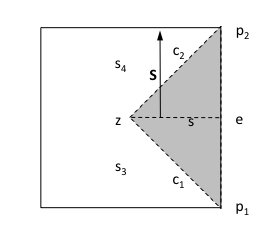
\includegraphics[width=0.40\textwidth]{side-maps.png}
    \caption{Various side map arrays supported by PENNANT.}
    \label{fig:side}
\end{figure}

The {\tt Mesh} class also has methods for computing other
geometry-related variables, such as edge and zone centers, lengths,
volumes, and surface vectors.  The surface vector for a side $s$, shown
by the vector {\bf S} in Figure~\ref{fig:side}, is used by force
computations in the hydro algorithms described later.

\subsection{Mesh generators}

PENNANT has internal mesh generation code that will generate three
different types of meshes, shown in Figure~\ref{fig:meshtype}.
\begin{figure}
    \centering
    \begin{tabular}{ccccc}
    
\includegraphics[width=0.25\textwidth]{rect-meshtype.png} &
    \hspace{0.025\textwidth} &
    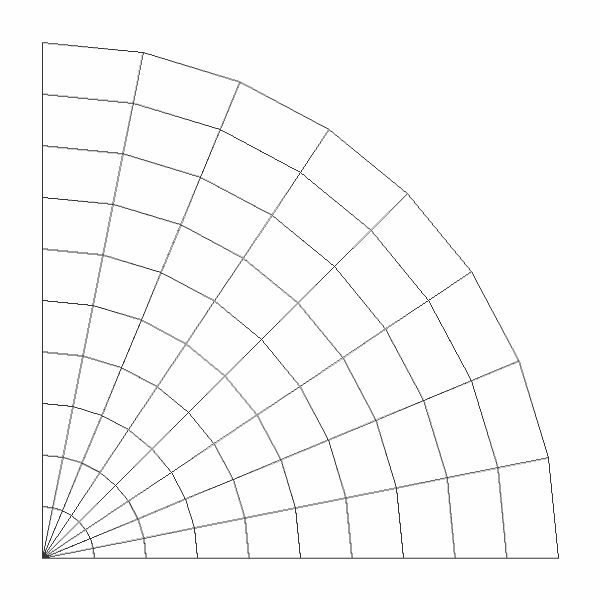
\includegraphics[width=0.25\textwidth]{pie-meshtype.png} &
    \hspace{0.025\textwidth} &
    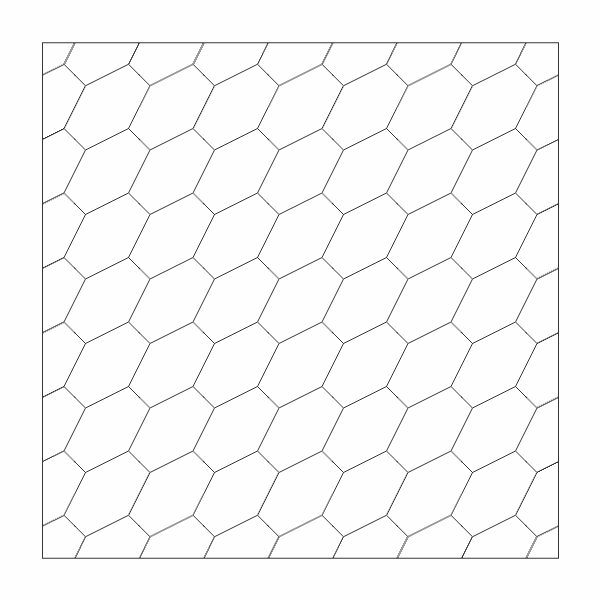
\includegraphics[width=0.25\textwidth]{hex-meshtype.png} \\
    (a) && (b) && (c) \\
    \end{tabular}
    \caption{Mesh types generated by PENNANT mesh generators:
    (a) {\tt rect}, (b) {\tt pie}, and (c) {\tt hex}.}
    \label{fig:meshtype}
\end{figure}

Note that the physics routines in PENNANT can process 2-D meshes of
any geometry; they are not limited to the mesh types shown here.
However, the internal mesh generators are set up to also generate domain
connectivity information needed by MPI (see section~\ref{sec:domain}),
which would be difficult to generate for arbitrary meshes.

\subsection{Chunk processing}
\label{sec:chunk}

The PENNANT {\tt Mesh} class has been set up to support computation on
chunks of the mesh in parallel.  This is used to implement OpenMP and CUDA
versions of the code and should lend itself to other task-based approaches
as well.  (MPI parallelism is implemented differently, using geometric
domain decomposition, as described in section~\ref{sec:domain}).
The maximum chunk size is controlled by the input file parameter
{\tt chunksize}.

In the current chunking approach, the lists of points and zones are
simply divided into chunks of size {\tt chunksize} (except for the final,
leftover chunk).  The list of sides is handled similarly, except that
the size of each individual chunk is rounded down slightly if necessary
so that each zone has all of its sides in the same chunk.  For each chunk,
the {\em first} and {\em last} indices of the chunk are stored.
(Note that {\em last} is actually one index beyond the end of the chunk,
in a similar manner to STL iterators, so that the sides in a side chunk
are those with $s_{first} \le s < s_{last}$.)  The total numbers of each
type of chunk ({\tt numXch}, where {\tt X} may be {\tt p}, {\tt s}, or
{\tt z}) are also stored.

Then, nearly all of the routines in the main hydro cycle have been
modified to take as input first and last indices of the appropriate
mesh entity.  This allows the hydro processing to be divided into
five phases, two on point chunks, two on side chunks, and one on zone
chunks.  Within each phase, all chunks are independent and can be
processed in parallel.
See {\tt Hydro::doCycle()} for the complete code flow.

A few of the helper routines, particularly in the {\tt QCS} class,
use scratch arrays the size of the chunk currently being processed.
The prefix {\tt s0} is used for an array with one entry per side
in the current chunk, with prefixes {\tt c0} and {\tt z0} used similarly
for corners and zones respectively.

\subsection{Domain decomposition}
\label{sec:domain}

The MPI implementation of PENNANT uses domain decomposition to put
a geometrically contiguous subset of the mesh on each processor.
It also generates information to allow point data to be communicated
across processors, as described below.

PENNANT follows FLAG in assigning each zone, corner and side to
a single MPI rank when decomposing the mesh.  However, any point on
a rank boundary is replicated on each rank which needs it; see
Figure~\ref{fig:decomp} for an illustration.  For any duplicated
point, one of its instances is designated as the {\em master}, and
the others are its {\em slaves}.  (The current PENNANT mesh generators
use the convention that the master point is the one on the
lowest-numbered MPI rank.)  When it is time to sum a quantity
from corners to points, the summation is first done for on-processor
corners in {\tt Mesh::sumOnProc}.  Then the summation is extended across
processors in three stages:

\begin{figure}
    \centering
    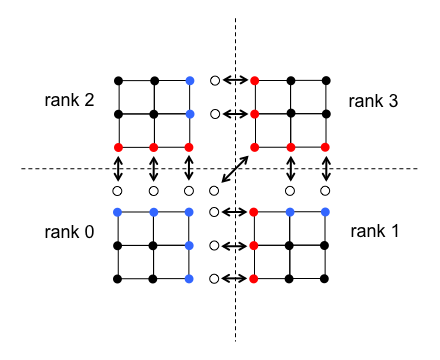
\includegraphics[width=0.6\textwidth]{domain-decomp.png}
    \caption{Example MPI decomposition of a mesh.  Master points are
        shown as blue, slaves as red, and proxies as white.
        MPI communications between slaves and proxies are shown
        as arrows.}
    \label{fig:decomp}
\end{figure}

\begin{enumerate}
    \item In {\tt Mesh::parallelGather},
        slave point values are assembled into messages, and sent
        to corresponding {\em proxy} points on the same rank as
        their masters (using MPI).
    \item In {\tt Mesh::parallelSum},
        master points sum their own values and all proxy values, and
        store sum at master and all proxies (on-processor only, no MPI
        is used).
    \item In {\tt Mesh::parallelScatter},
        the updated proxy point values are assembled into messages
        and sent back to their corresponding slave points (using MPI).
\end{enumerate}


\section{Physics details}

\subsection{Basic hydro algorithms}

PENNANT provides a subset of the compatible Lagrangian staggered grid
hydrodynamics (SGH) algorithms implemented in FLAG and described
in~\cite{hydro}.  These are implemented in the {\tt Hydro} class.
An outline of the main steps is given in Table~\ref{tbl:dataflow}.

\def\RR{\raggedright}

\begin{table}
\caption{Basic data flow for FLAG/PENNANT hydrodynamics.}
\label{tbl:dataflow}
\begin{tabular}{lp{108pt}p{180pt}}
    \hline
    step & main inputs & main outputs \\
    \hline
    Predictor step: \\
    1. Update mesh & point velocity, position & point position (half-advanced) \\
    1a. Update mesh geometry & point position & {\bf {\RR side and zone volume; zone density; \\ side surface vector } } \\
    2. Compute point masses & {\RR zone density, volume; \\ side mass fraction} & {\bf point mass} \\
    3. Update thermodynamic state & {\RR zone density, specific\\ energy, work rate} & zone pressure, sound speed \\
    4. Compute forces & {\RR side surface vector; \\ zone pressure} & side and {\bf point force} \\
    4a. Apply boundary conditions & point force, velocity & point force, velocity (constrained) \\
    5. Compute accleration & point force & point acceleration \\
    \hline
    Corrector step: \\
    6. Update mesh & {\RR point acceleration, \\ velocity, position} & point velocity, position (fully advanced) \\
    6a. Update mesh geometry & point position & {\bf side and zone volume} \\
    7. Compute work & {\RR point position, velocity; \\ side force} & {\bf zone work, work rate, total energy} \\
    8. Update zone state variables & {\RR zone volume, mass,\\ total energy} & zone density, specific energy \\
    \hline
\end{tabular}
\end{table}

The PENNANT hydro algorithm is a {\em Lagrangian} method, meaning that
the computational mesh moves with the material as the problem state
advances.  This implies that the mass and material type within each zone
are constant throughout the problem, but the zone's position and shape
will change over time.

It is also a {\em staggered-grid} method, meaning that mesh positions and
related variables (velocity, acceleration, etc.) are stored on points,
while most state variables (density, energy, pressure, etc.) are stored
on zones.  Therefore, the calculation must frequently use values of
zone-based variables to compute point-based results, or vice-versa.
In Table~\ref{tbl:dataflow}, such results are shown in {\bf bold}.
(Note that this is true for five of the 11 steps shown.)

To facilitate these calculations, many of the calculation loops are done
over sides, and some intermediate variables are stored on sides.
This works since each side can be easily correlated to its
corresponding zone and points using the mapping arrays in the {\tt Mesh}
object.  A few routines use corners in a similar manner.

PENNANT hydro uses a {\em predictor-corrector} time integration
method.  Each cycle can be broken into two steps, shown in the table.
The cycle begins with all problem state defined for the beginning of the
timestep.  In the predictor step, some variables are advanced to the
middle of the timestep, in order to compute half-advanced point
acceleration values.  In the corrector step, the new accelerations are
then used to advance all variables to the end of the timestep.

To implement the predictor-corrector scheme, it is necessary to store
multiple values of some of the problem variables.  This is done
using the following notation convention:
\begin{itemize}
\item suffix $0$ = the beginning of the timestep (``cycle n'')
\item suffix $p$ = half-way through the timestep (``cycle n + 1/2'')
\item no suffix = completion of the timestep    (``cycle n + 1'')
\end{itemize}
Some examples are shown in Table~\ref{tbl:timestep}.
Note that some entries in the table are blank, since not all quantities
are needed at all times.

\begin{table}
\centering
\caption{Examples of PENNANT variables and their dependence on timestep.}
\label{tbl:timestep}
\begin{tabular}{lccc}
    \hline
    & \multicolumn{3}{c}{Part of time step} \\
    quantity & begin & middle & end \\
    \hline
    point coordinate       & px0   & pxp     & px \\
    point velocity         & pu0   &         & pu \\
    point acceleration     &       & pap \\
    point force            &       & pf \\
    point mass             &       & pmaswt \\
    \\
    zone center coordinate &       & zxp     & zx \\
    zone mass              &       &         & zm \\
    zone volume            & zvol0 & zvolp   & zvol \\
    zone density           &       & zrp     & zr \\
    zone specific energy   &       &         & ze \\
    \\
    side volume            &       & svolp   & svol \\
    side surface vector    &       & ssurfp \\
    \hline
\end{tabular}
\end{table}

\subsection{Material model}

PENNANT provides finite-volume, arbitrary-polygon cells with a
gas material model, implemented in the {\tt PolyGas} class.
This class includes code to compute a simple gamma-law gas
equation of state, and to compute the resulting pressure-based
forces.

\subsection{Subzonal pressures}

PENNANT provides the Temporary Triangular Subzoning (TTS) algorithm
described in~\cite{szp,tts}.  This is implemented in the {\tt TTS}
class.  This prevents certain kinds of distortions of zones, such as
``hourglassing,'' by estimating a pressure for each side, and adding
a force to each side based on the difference
between the zone and side pressures.

Note to FLAG users:  The FLAG implementation of TTS contains, in addition
to the subzonal pressure treatment, an artificial viscosity algorithm
based on the subzonal pressures; the artificial viscosity is not part of
the standard TTS description in the references.  Only the subzonal pressure
part of TTS is implemented in PENNANT.

\subsection{Artificial viscosity}

PENNANT provides the tensor artificial viscosity algorithm of Campbell and
Shashkov, described in~\cite{qcs}.  This is implemented in the {\tt QCS}
class.  (The symbol $q$ is traditionally used to denote artificial
viscosity, hence the {\tt Q} prefix on the class name.)
Artificial viscosity is a fictitious term commonly introduced into
fluid flow equations to correctly handle
shock regions with large discontinuities in
the problem state variables.


\section*{Acknowledgements}

Thanks to Mikhail Shashkov and the ASCR ``Mimetic Methods for PDEs''
project, and the ASC Hydrodynamics project, for providing support for
this work.  Thanks to Pat McCormick and the ASC Programming Models
project for providing some additional support for development of the
MPI version.

Thanks also to the Lagrangian Applications Project members who have
contributed to the FLAG code; parts of the PENNANT code and documentation
are adapted from their work.
And finally, thanks to the participants in the Intel EPOCH workshop
in the summer of 2012; several optimization ideas from that workshop
have been incorporated into subsequent PENNANT versions.


\begin{thebibliography}{9}
\bibliographystyle{alpha}

\bibitem{leblanc}
D.J.~Benson.
\newblock Momentum advection on a staggered mesh.
\newblock {\em J. Comput. Phys}, 100:143--162, 1992.

\bibitem{qcs}
J.~Campbell and M.~Shashkov.
\newblock A tensor artificial viscosity using a mimetic finite difference
  algorithm.
\newblock {\em J. Comput. Phys}, 172:739--765, 2001.

\bibitem{hydro}
E.J. Caramana, D.E. Burton, M.~Shashkov, and P.P. Whalen.
\newblock The construction of compatible hydrodynamics algorithms utilizing
  conservation of total energy.
\newblock {\em J. Comput. Phys.}, 146:227--262, 1998.

\bibitem{szp}
E.J. Caramana and M.J. Shashkov.
\newblock Elimination of artificial grid distortion and hourglass-type motions
  by means of {L}agarangian subzonal masses and pressures.
\newblock {\em J. Comput. Phys.}, 142:521--561, 1998.

\bibitem{noh}
W. F. Noh,
\newblock Errors for calculations of strong shocks using an artificial viscosity and an artificial heat flux.
\newblock {\em J. Comput. Phys.}, 72:78, 1987.

\bibitem{sedov}
L. I. Sedov,
\newblock Similarity and Dimensional Methods in Mechanics.
\newblock Academic Press, New York, 1959.

\bibitem{tts}
K.B. Wallick.
\newblock Temporary triangular subzoning ({TTS}), in {REZONE}: A method for
  automatic rezoning in two-dimensional lagrangian hydrodynamics problems.
\newblock {Technical {R}eport LA-10829-MS}, Los Alamos National Laboratory, Los
  Alamos, NM 1987.

\end{thebibliography}


\appendix
\section{Version Log}

\begin{description}
\item[0.6] February 2014 \\
     First MPI version.  MPI capability is working and mostly
     optimized; MPI+OpenMP is working but needs optimization.
     Replaced GMV mesh reader with internal mesh generators.
     Added QCS velocity difference routine to reflect a recent
     bugfix in FLAG.  Increased size of big test problems.

\item[0.5] May 2013 \\
     Further optimizations.

\item[0.4] January 2013 \\
     First open-source release.  Fixed a bug in QCS and added some
     optimizations.  Added Sedov and Leblanc test problems, and some
     new input keywords to support them.

\item[0.3] July 2012 \\
     Added OpenMP pragmas and point chunk processing.  Modified physics
     state arrays to be flat arrays instead of STL vectors.

\item[0.2] June 2012 \\
     Added side chunk processing.  Miscellaneous minor cleanup.

\item[0.1] March 2012 \\
     Initial release, internal LANL only.
\end{description}

\section{Copyright and License Information}

Copyright \copyright 2012, Los Alamos National Security, LLC.
All rights reserved.

Copyright 2012. Los Alamos National Security, LLC.
This software was produced under U.S. Government contract
DE-AC52-06NA25396 for Los Alamos National Laboratory (LANL), which is
operated by Los Alamos National Security, LLC for the U.S. Department
of Energy. The U.S. Government has rights to use, reproduce, and
distribute this software. NEITHER THE GOVERNMENT NOR LOS ALAMOS
NATIONAL SECURITY, LLC MAKES ANY WARRANTY, EXPRESS OR IMPLIED, OR
ASSUMES ANY LIABILITY FOR THE USE OF THIS SOFTWARE. If software is
modified to produce derivative works, such modified software should be
clearly marked, so as not to confuse it with the version available from
LANL.

Additionally, redistribution and use in source and binary forms, with
or without modification, are permitted provided that the following
conditions are met:

\begin{enumerate}
\item Redistributions of source code must retain the above copyright
   notice, this list of conditions and the following disclaimer.
\item Redistributions in binary form must reproduce the above
   copyright notice, this list of conditions and the following
   disclaimer in the documentation and/or other materials provided
   with the distribution.
\item Neither the name of Los Alamos National Security, LLC, Los Alamos
   National Laboratory, LANL, the U.S. Government, nor the names of its
   contributors may be used to endorse or promote products derived from
   this software without specific prior written permission.
\end{enumerate}

THIS SOFTWARE IS PROVIDED BY LOS ALAMOS NATIONAL SECURITY, LLC AND
CONTRIBUTORS ``AS IS'' AND ANY EXPRESS OR IMPLIED WARRANTIES, INCLUDING,
BUT NOT LIMITED TO, THE IMPLIED WARRANTIES OF MERCHANTABILITY AND FITNESS
FOR A PARTICULAR PURPOSE ARE DISCLAIMED. IN NO EVENT SHALL LOS ALAMOS
NATIONAL SECURITY, LLC OR CONTRIBUTORS BE LIABLE FOR ANY DIRECT,
INDIRECT, INCIDENTAL, SPECIAL, EXEMPLARY, OR CONSEQUENTIAL DAMAGES
(INCLUDING, BUT NOT LIMITED TO, PROCUREMENT OF SUBSTITUTE GOODS OR
SERVICES; LOSS OF USE, DATA, OR PROFITS; OR BUSINESS INTERRUPTION)
HOWEVER CAUSED AND ON ANY THEORY OF LIABILITY, WHETHER IN CONTRACT,
STRICT LIABILITY, OR TORT (INCLUDING NEGLIGENCE OR OTHERWISE) ARISING
IN ANY WAY OUT OF THE USE OF THIS SOFTWARE, EVEN IF ADVISED OF THE
POSSIBILITY OF SUCH DAMAGE.

\end{document}
